\chapter{Overall Description}
\section{Product Perspective}
\subsection{Scenarios}

\subsubsection{Creating a tournament}
Chip, a professor of Algorithm and Data Structures at Mouseton Institute of Technology, prepared to teach the chapter on strings, launching the "Strings Operations" coding tournament on CKB.
To expand participation, he allowed his colleague Dale to create challenges for his software engineering class.
Students across classes would compete in string manipulation tasks, ranging from basic concatenation to advanced text analysis, fostering collaboration and learning.
To make the tournament more interesting, Chip decided to award badges to the best performing students, so he adds th badge for the student who participated in the most tournaments, the one for the student who won the most battles and the one for the student that wrote the most lines of code.
All students already subscribed to CKB were notified of the new tournament, and they could join it from the tournament page.

\subsubsection{Creating a battle}
In order to get the students familiar with the CKB platform and its features, Chip created an easy battle for his students to practice on, called "wordcheck", that basically requires the student to implement the game wordle, to be implemented in c language.
He decides that the battle will last 2 weeks and that the students will be able to work in teams of 2 or 3 people; they will be able to join the battle until the last day of the battle.
In addiction, he wants to give extra points to the code cleanup, so he will have to revise the code of each team at the end of the battle and assign extra points to the teams that wrote clean code.
He sets all this information in the battle creation form and then he creates the battle.

\subsection{Creating Game badges}
Scrooge, a professor of Algorithm and Data Structures at Duckburg University, thinks that, in addiction to the badges that are already present in the CKB platform, it would be nice to have also a badge for the student who reaches the perfect score in a battle and a badge for the student who reaches the perfect score in a tournament.
Since the CKB platform allows educators to create new badges, he creates the two badges and from now on, all educators will be able to include such badges in their tournaments and battles.

\subsubsection{Joining a battle}
Huey and Dewey, two students of Chip's class, are notified of a new battle and decide to join it.
Since the the more the merrier, they decide to invite their friend Louie to join them in the battle.
Louie receives the invitation mail and decides to join the battle in their team.
After the registration deadline, they are notified that the battle is about to start and they are given the link to the GitHub repository of the battle to fork and set up the automated workflow in order to be able to link their GitHub account to the CKB platform.
After the automated workflow is set up, they are ready to start working on the battle.

\subsubsection{Improving the score and obtaining a badge}
Donald is a warrior of the "wordcheck" battle and he is working on the battle alone.
After a fitst commit, he logs in to the CKB to check his score.
He sees that he is in the 3rd position and that he is 10 points behind the leader group, that is composed by Huey, Dewey and Louie.
Fortunately, the battle is still open and the CKB platform allows him to improve his score by pushing new commits to the GitHub repository, so he decides to work on the battle for a couple of days and then push his work to the GitHub repository.
After checking his score again, he sees that he is now in the 1st position and moreover he obtained a badge for being the first to reach 100 points in the battle and now both students and professors can see this badge when they visit Donald's profile.

\subsubsection{Closing a battle}
When the deadline for the battle created by Scrooge is reached, all participants are notified that the battle is closed and that they can't push new commits to the GitHub repository.
Scrooge is notified that the battle is closed and he can now evaluate the code of each team and assign extra points for the clarity of the comments and the code, as he decided when he created the battle.
After the evaluation, the final rank of the battle is available to all participants and the students are notified that they can now see the final rank of the battle.

\subsubsection{Closing a tournament}
Chip decides to close the "Strings Operations" tournament, even if the deadline is not reached yet.
In order to do so, he logs in to the CKB platform and he closes the tournament.
All participants are notified that the tournament is closed and that they can't join it anymore, in the end, the CKB platform makes the final rank of the tournament available to all participants.

\subsubsection{Accessing the scores of the players}
Huey wishes to enroll to the class of Advanced Algorithms and Data Structures held by professor Pippo, so he applies for the class.
Pippo, who wants to make sure that Huey is a good student, comes to know that Huey is a very active user of the CKB platform and he decides to check his profile.
He sees that Huey has a very high score in the "Strings Operations" tournament and that he has a badge for being the most active user of the platform and he also notes that Huey is involved in more than one tournament simultaneously.
Thanks to the CKB platform, Pippo has now a complete overview of Huey's skills and he can decide whether to accept his application or not.

\subsection{Class Diagram}
In figure \ref{fig:software-class-diagram} is represented the class diagram of the software. In particular, the most important details are :
\begin{itemize}
    \item There are only two possible types of users : the Student type and the Educator type;
    \item The Educator can create tournaments and battles, he can grants other educators to his own tournament;
    \item The Student can invite other students, he can achieves some badges, he can subscribes to a tournament and he will use GitHub. But the most important detail is the one about subscribing to a battle : in fact, a student can subscribe to a battle by creating is own team (a team is composed by at least one person) or by joining an existing team. In this way we don't use a "Team" class because a team doesn't exist without a battle;
    \item The Tournament and Battle classes use the MailAPI to notify students about events.

\end{itemize}
\begin{figure}[H]
    \centering
    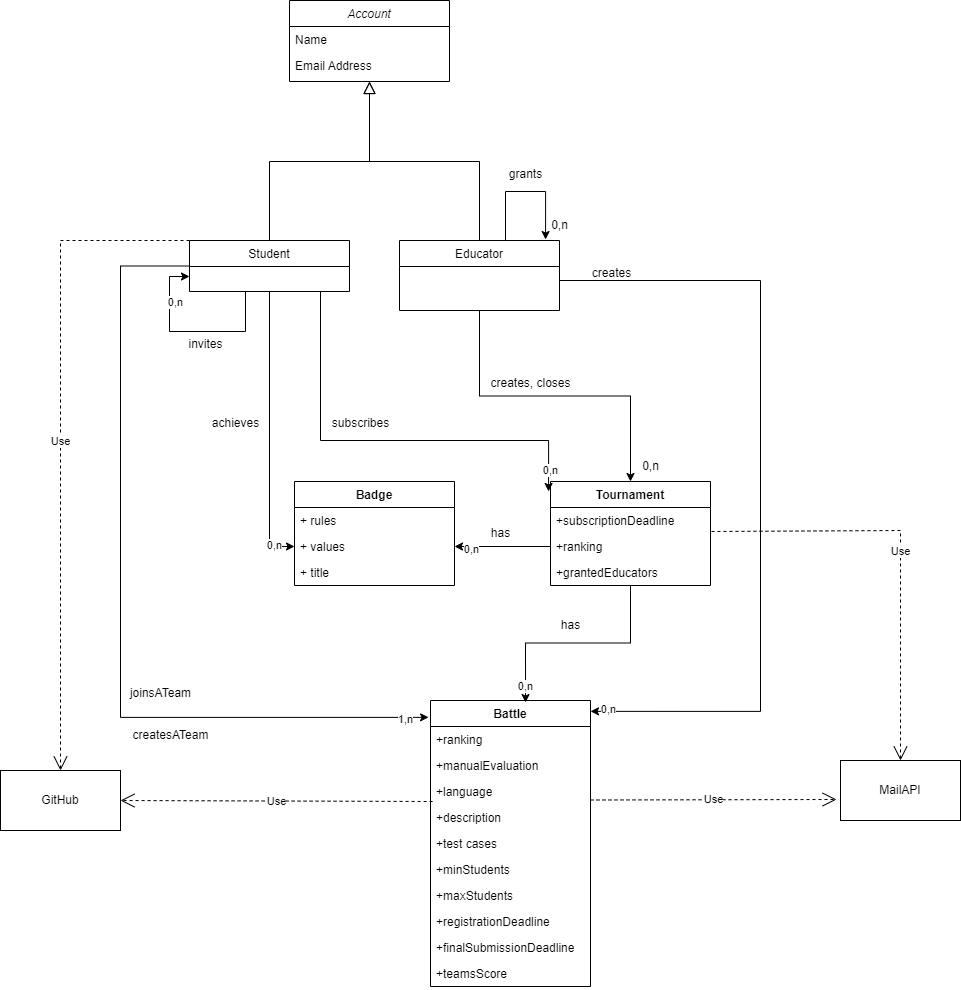
\includegraphics[width=0.8\textwidth]{images/state_diagrams/ClassDiagram.png}
    \caption{Software Class Diagram}
    \label{fig:software-class-diagram}
\end{figure}

\subsection{State Diagrams}
The following state diagrams describe the life cycle of the main entities of the system.
Moreover, they also specify the sequence of states that an object goes through during its lifetime in response to stimuli from the environment.
We want to focus on the events that cause a transition from one state to another and the actions that result from a state change.

\subsubsection*{Tournament}
After an educator creates a tournament, it is both in the \textit{registration open} and \textit{tournament open} states.\\
In the \textit{registration open} state, students can join the tournament, while in the \textit{tournament open} state, educators with the right permissions can create battles within the tournament, and that leads the tournament to the \textit{battling} state.\\
When the deadline for the registration is reached, the tournament moves to the \textit{registration closed} state and no more students can join it.\\
When the deadline for the registrations is reached, no more students can join the tournament and it moves permanently to the \textit{registration clcsed} state.\\
During the \textit{battling} state educatos can start multiple parallel battles and, if and only if all battles are ended, the educator can finally close the tournament.\\
The diagram is shown in figure \ref{fig:tournament-state-diagram}.

\subsubsection*{Battle}
The battle evolves in a linear way, starting from the \textit{registration opem} immediately followed by the \textit{registration closed} state.\\
After the registration deadline is reached, the github repository of the battle is created and thus the battle moves to the \textit{coding} state, allowing the students to fork the repository and start working on the battle.\\
When the deadline for the battle is reached, the educators can start evaluating the code of the students, if previously enabled (\textit{consolidation} state). \\
After the evaluation is completed, the battle can be closed and the final rank is available to all participants.\\
The diagram is shown in figure \ref{fig:battle-state-diagram}.

\subsubsection*{Score evaluation}
The score evaluation of a battle is a process that is triggered by the end of a battle and it is composed by multiple steps.\\
First, three aspects can be automatically evaluated: functional aspects (the higher the better, +), timeliness (the lower the better, -) and quality level of the sources, extracted through static analysis tools (+). \\
Finally, if the educator enabled the manual evaluation, he can assign extra points. \\
The diagram is shown in figure \ref{fig:score-evaluation-state-diagram}.

\begin{figure}[H]
    \centering
    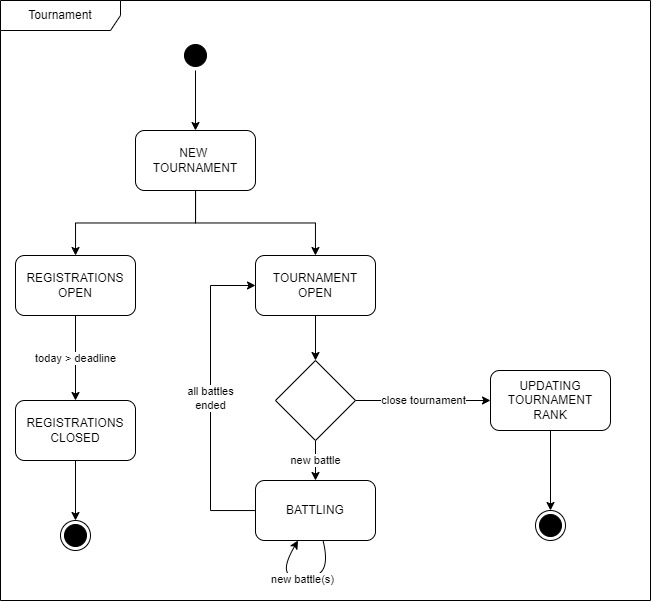
\includegraphics[width=.8\textwidth]{images/state_diagrams/tournament.jpg}
    \caption{Tournament state diagram}
    \label{fig:tournament-state-diagram}
\end{figure}
\begin{figure}[H]
    \centering
    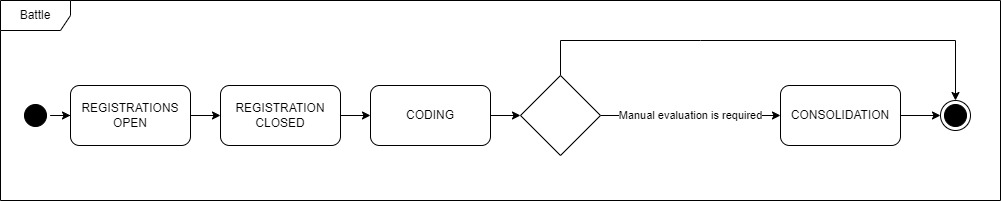
\includegraphics[width=1\textwidth]{images/state_diagrams/battle.jpg}
    \caption{Battle state diagram}
    \label{fig:battle-state-diagram}
\end{figure}
\begin{figure}[H]
    \centering
    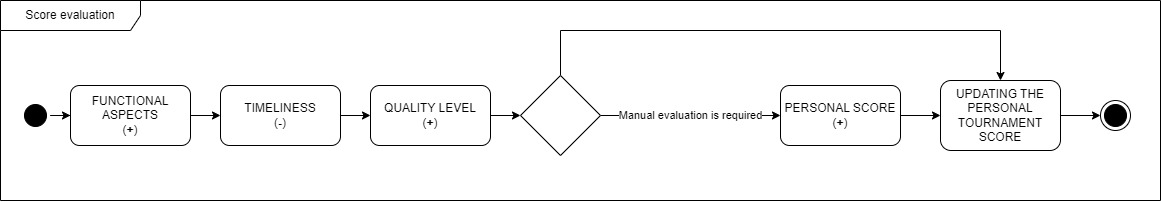
\includegraphics[width=1\textwidth]{images/state_diagrams/score_evaluation.jpg}
    \caption{Score evaluation state diagram}
    \label{fig:score-evaluation-state-diagram}
\end{figure}

{\color{orange}
\section{Product Functions}
\subsection{Registrater function}
- Studente o educatore
- Educatore ha un livello di accout maggiore rispetto allo studente -> Crea battaglie o tornei e specifico i dettagli per ogni cosa

\subsection{Creating tournament function}
- Come si crea il torneo molto in generale

\subsection{Creating battles function}
- Come si crea la battaglia molto in generale

\subsection{Partecipating in tournament and battles function}
- Come si iscrive a battaglie e tornei molto in generale

\subsection{Score visualization function}
- Score, ranking e badges vederli

\subsection{Gamification function}

\section{User characteristics}
Users of the system fall into one of the following categories: student or educator.

\subsection*{Student}
Identifies a person who provides instruction or education, such as a teacher.

\subsection*{Educator}
}


\section{Assumptions, Dependencies and Constraints}

\subsection{Domain Assumptions}
\newlist{assumptionsenumerate}{enumerate}{1}
\setlist[assumptionsenumerate,1]{label=\textbf{D}\arabic*., ref=D\arabic*}
\begin{assumptionsenumerate}
    \item STUs code with the programming language setted for the battle to which they are partecipating
    \item EDUs upload the code kata with the description and the correct software project, including test cases and build automation scripts
    \item STUs fork the GitHub repository of the code kata and set up an automated workflow through GitHub Actions that informs the CKB platform (through proper API calls) as soon as STUs push a new commit into the main branch of their repository
    \item EDUs manual evaluation range from 0 to 100\footnote{The full evaluation will be given by the average of all the four aspects evaluated by the CKB platform, the three automatic ones and the manual one}
    \item The information inserted at registration moment of all users are truthful
    \item GitHub and the tool for static analysis work properly
    \item A team is formed by at least one person
    \item All users subscribed to the CKB platform have a GitHub account
\end{assumptionsenumerate}

\subsection{Dependencies}
\begin{table}[H]
    \centering
    \renewcommand{\arraystretch}{1.5}
    \begin{tabular}{l l p{11.5cm}}
        \hline
        \textbf{Dep1} &  & The system will require internet connection to interact with CKB and other users           \\
        \textbf{Dep2} &  & The system will integrate an external API in order to compile the code written by students \\
        \textbf{Dep3} &  & The system will integrate a GitHub API in order create repository for each battle          \\
        \hline
    \end{tabular}
    \caption{Dependencies}
\end{table}

\subsection{Constraints}

\begin{itemize}
    \item The software must follow local laws and rules, especially when it comes to handling user data, like letting users access their data when they want.
    \item The software should only collect the data it really needs, like just the user's email address.
    \item To keep users' important info safe, like passwords and personal data, it must be stored in SHA256 encoding in the database.
    \item When choosing external APIs, especially those that are crucial for it to work properly, we should pick the ones that are the most dependable and always available.
\end{itemize}